\chapter{Concept}
\label{Concept}


Based on the analysis in chapter \ref{relatedwork} the navigation stack seems to be a well fitting core structure for the navigation. As mentioned, there have not yet been any publications of using it for the navigation of a Carolo-Cup vehicle, making the following analysis mandatory. 

This analysis of the recommended navigation stack setup and potentially needed modifications are covered in this chapter, aswell as a resulting concept.
T
\section{Analysis of the Recommended Setup}
The recommended setup shown in figure \ref{recnavsetup} needs to be checked for compatibility with the specific use case.

\begin{figure}[H]
	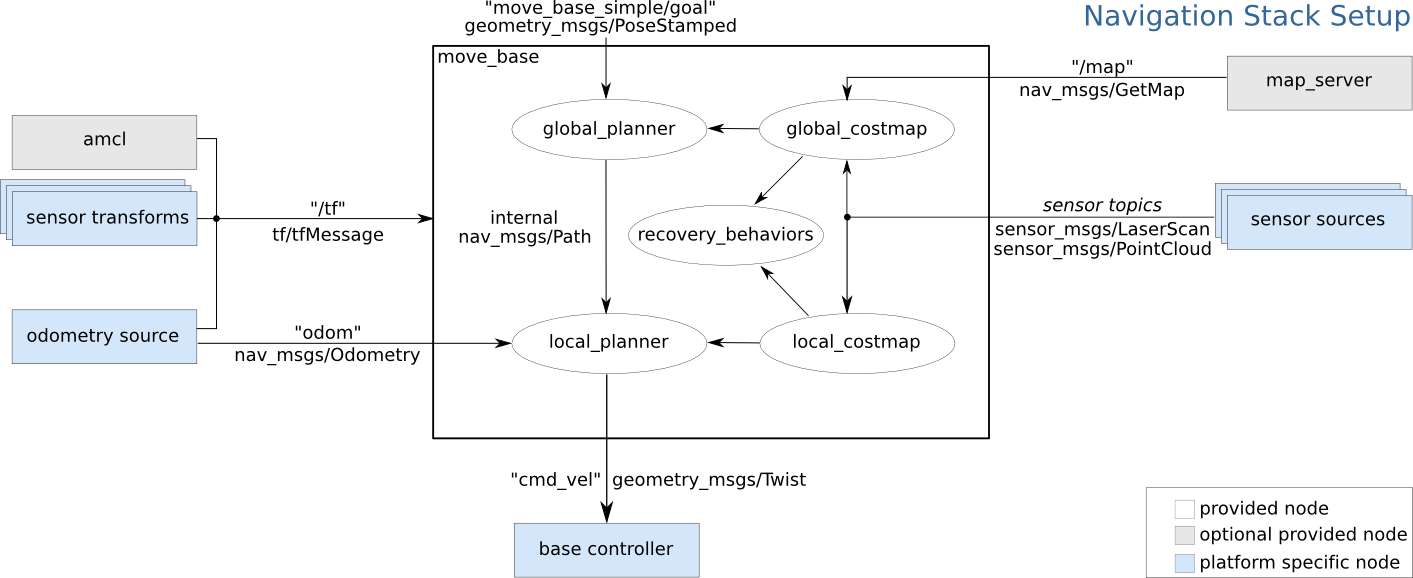
\includegraphics[width=\textwidth]{Pictures/navigation stack setup}
	\caption{Recommended navigation stack setup}
	\label{recnavsetup}
\end{figure}

The following points highlight needed modifications and configurations that allow the usage of the navigation stack.

\begin{itemize}
	\item In the Carolo-Cup the environment is totally unknown at the start. Therefore the map\_server and amcl can not be used in this thesis, since they rely on a prerecorded map.
	\item The blue nodes in the setup contain the platform specific nodes. Hence they have to be configured and selected according to the setup of the Arlo robot platform.
	\item The setup contains no node that supplies a goal, which is necessary for autonomous navigation.
	\item To achieve the required navigation behavior specified in chapter \ref{requirements} the components of move\_base have to be selected and configured accordingly.
	\item The raw sensor data in a realistic use case is influenced by noise, introducing the need for filtering.
	\item The navigation stack and its components receive data in very specific formats. Therefore, nodes for data processing and conversion have to be added to the structure.
\end{itemize}

The highlighted problems will be discussed in the following sections.



\subsection{PoseFinder}

This node has the task of constructing a goal for the navigation, based on the sensor data or a map.

The road detection is only able to detect the road to a certain distance. Everything beyond is unknown. 
To allow the planners to generate smooth paths the distance, at which goals need to be found should be relatively far away from the robot.
For uninterrupted navigation, this node needs to continuously find new goals and send them to move\_base

Finding a goal based on sensor data is redundant, if a map including the road is available. This allows larger distances, at which goals can be found. Based on sensor noise, this is likely to be more precise as well.

\subsection{Map}
As described amcl and the map\_server can not be used in this scenario.

To replace these nodes, a SLAM (simultaneous localization and mapping) algorithm can be used.
This is possible, since the robot might drive multiple rounds, allowing it to build its own map.\\

The SLAM algorithm can be used to determine the robots position relative to the map, by providing a transformation between the ``map'' and ``odom'' tf\_frames. Furthermore the map can be used to define go and no-go zones.

Unfortunately, the data that can be fed to the SLAM algorithm is very limited, since it is not guaranteed, that the lidar sensor always sees static obstacles. Another data source for the SLAM algorithm could be the points extracted from the road detection. Unfortunately, the road markings are similar to a corridor and do not have a lot of features, other than the curvature of the road.\\

\begin{figure}[H]
	\centering
	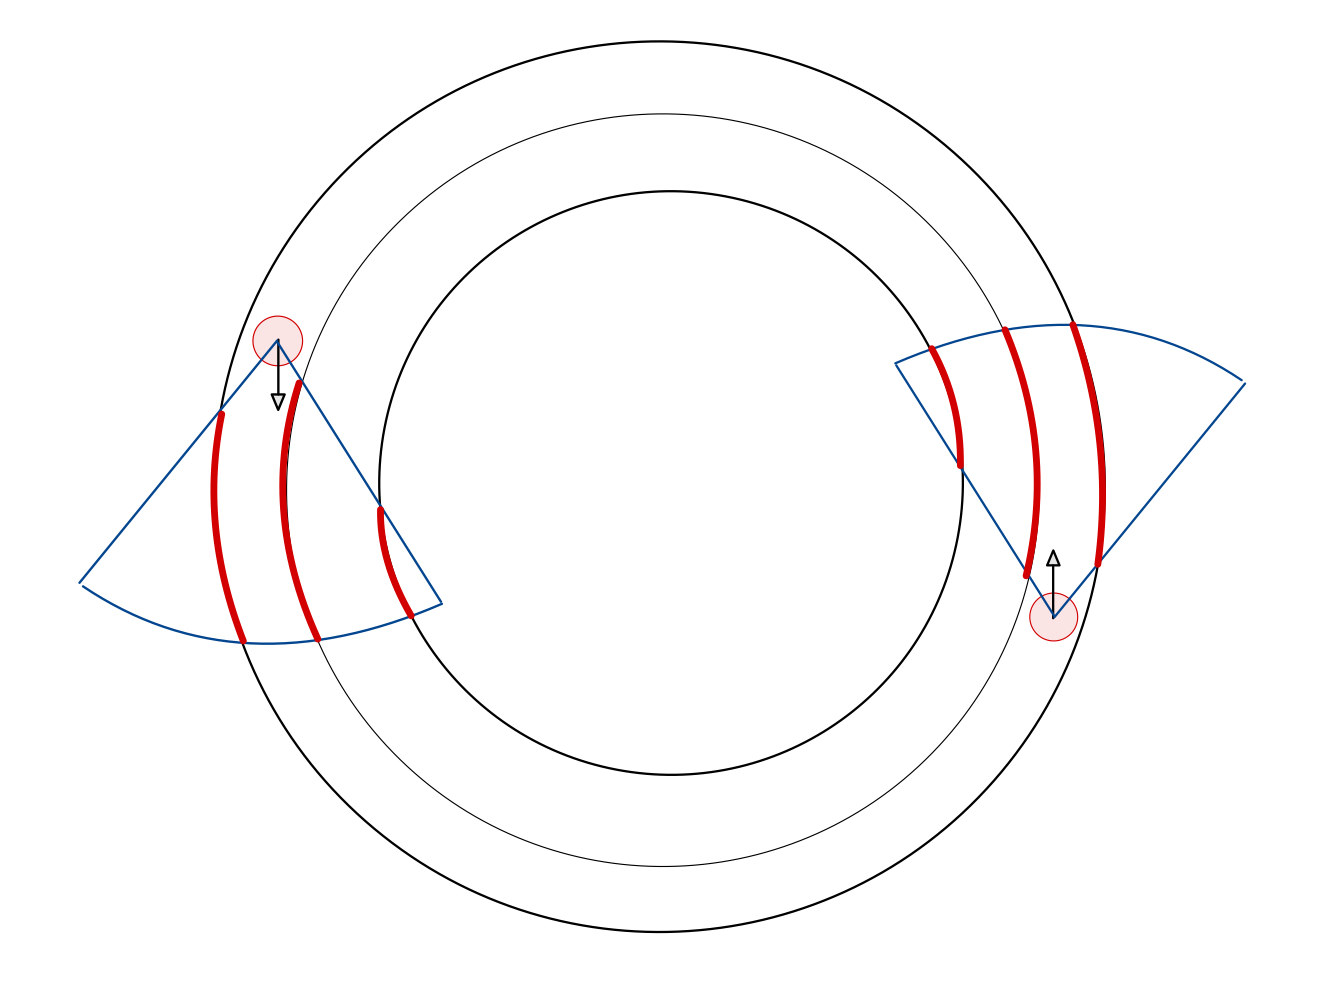
\includegraphics[width=.5\textwidth]{Pictures/selfsimillar}
	\caption{Visualization of self similar data}
	\label{selfsimilar}
\end{figure}

This significantly decreases the reliability of the map which therefore will highly depend on good odometry, since for example a straight section of the road always looks similar, even if it is on the other side of the circuit like pictured in \ref{selfsimilar}. The odometry provides an estimate, where the SLAM algorithm should attach the sensor data to the map.

To get a better map, both of the data inputs have to be used, which results in the need of a SLAM algorithm with multiple sensor inputs.\\

\subsection{Sensor Transforms}

As pictured in figure \ref{recnavsetup} the navigation stack requires transformations between the sensor specific frames, the base frame of the robot and its odometry frame. This results in the tf\_tree of the robot.

This can be realized by calculating the transformations between the frames manually. However, the ROS package robot\_state\_publisher is a cleaner approach. This requires a robot description in URDF format, that specifies the relations between everything mounted on the robot.\\

The required transform from the base to the odom frame is built by using the position derived from the wheel encoder data.

\subsection{move\_base}

move\_base consists of a global and a local part, the combination of both defines the path finding characteristic of the navigation. 
To define requirements for the internal nodes, they will be categorized into a global and a local stage.

\subsubsection{Global Stage}
The general task of the global planner is like described in the theoretical background to plan a rough path through the grid of the costmap, that does not collide with any lethal cell.\\

In this scenario the global planner will also be used to guide the robot on the correct lane. This results in the following requirements:

\begin{itemize}
	\item The global costmap needs information about the road markings and the obstacles detected by the lidar scan.
	\item The global costmap needs to incorporate cost that generate a preference for the right lane, but allow the global path to go to the left lane in case of an obstacle.
	\item The global planner has to respect all cost values.
\end{itemize}

\subsubsection{Local Stage}
The local stage on the other hand has the task of finding a path, that is feasible for the dynamics of the robot and does not collide with objects.\\
This path is supposed to be close to the global path and follow its lane changes, but it needs to be able to separate itself from it, if necessary.

Therefore, the local costmap needs to contain information about the road markings and the obstacles detected by the lidar scan.


\subsection{Sensor Filter}

This block incorporates the nodes that process the sensor data into a format, that is usable for the navigation\_stack. 
Therefore, it consists out of the following nodes:

\begin{itemize}
	\item \textbf{roadDetection} will extract approximated polynomials for the road markings and the lanes from the camera data
	\item \textbf{markfreespace} needs to publish point clouds to the costmaps and the SLAM algorithm consisting of the road detection data and the lidar scan.
\end{itemize}

As described in the requirements, the simulator is supposed to produce realistic sensor data, which might need filtering. These filters are additionally located in this block.

\section{Resulting Concept}
The schematic in figure \ref{navconcept} shows the concept of the navigation.  To keep the schematic as simple as possible, not every connections between the nodes are highlighted (Appendix \ref{config} shows the finalized schematic).\\

\begin{figure}[H]
	\begin{center}
		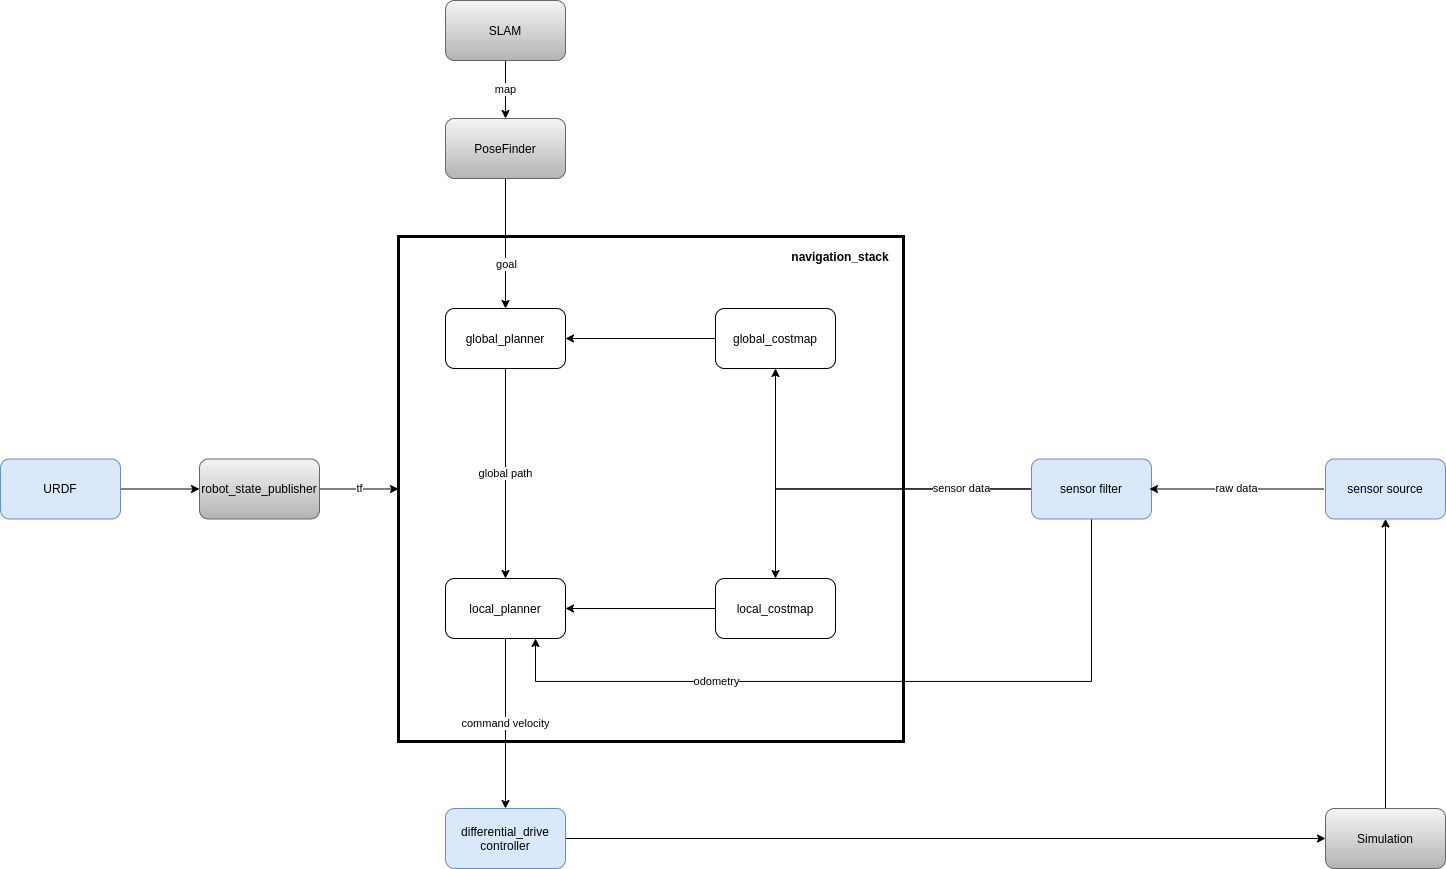
\includegraphics[width=140mm]{Pictures/Updated navigation concept}
		\caption[Updated navigation concept]{Updated navigation concept (Blue - platform specific nodes, Grey - optional nodes, White - move\_base nodes)}
		\label{navconcept}
	\end{center}
\end{figure}



The PoseFinder will repeatedly find goals based on the current state of the map and the sensor data. The goals will then be handed over to the navigation stack. This uses the filtered sensor data to determine, where the robot is as well as, where it is allowed to go and where not. Afterwards the cascading planners produce first a rough, collision free, path on the correct lane and then a path that is possible for the dynamics of the robot. This path then gets converted to velocity commands and sent to the motor controller.\\




